\documentclass[a4paper,11pt,exos]{nsi} % COMPILE WITH DRAFT
\usepackage{pifont}
\usepackage{fontawesome5}
\geometry{margin=2cm}




\begin{document}
\classe{\terminale Comp}
\titre{Corrigé de l'évaluation-bilan 3 bis}
\maketitle

\exo{}
\begin{enumerate}
    \item Soit $f$ la fonction définie sur $I=\fif{0}{40}$ par $\quad f(x)=(10x-10)e^{-0,1x}$.
    \begin{enumalph}
        \item Calculer $f(0)$ et $f(40)$.
        \item Démontrer que pour tout $x\in I, \quad f'(x)=(11-x)e^{-0,1x}$.
        \item Dresser le tableau de variations de la fonction $f$ sur $I=\fif{0}{40}$.
        \item Démontrer que l'équation $f(x)=20$ admet exactement deux solutions sur l'intervalle $\fif{0}{40}$.
    \end{enumalph}
    \textcolor{UGLiBlue}{
        \begin{enumalph}
            \item \begin{multicols}{2}
                \begin{tabbing}
                    $f(0)$  \= $=(10\times 0-10)e^{-0,1\times 0}$\\
                    \> $=-10\times 1$\\
                    \> $=-10$
                \end{tabbing}
                \begin{tabbing}
                    $f(40)$  \= $=(10\times 40-10)e^{-0,1\times 40}$\\
                    \> $=(400-10)e^{-4}$\\
                    \> $=390e^{-4}$\\
                    \> $\approx 7,14$
                \end{tabbing}
            \end{multicols}
            \item Soit $x\in\fif{0}{40}$
            \begin{tabbing}
                $f'(x)$ \= $=10e^{-0,1x}+(10x-10)\times (-0,1)e^{-0,1x}$\\
                \> $=10 e^{-0,1x}+(-x+1)e^{-0,1x}$\\
                \> $=(10-x+1)e^{-0,1x}$\\
                \> $=(11-x)e^{-0,1x}$
            \end{tabbing}
            \item Pour tout $x\in\fif{0}{40}$, $e^{-0,1x}>0$.\\
            Donc $f'(x)$ est du signe de $(11-x)$.
            \begin{multicols}{2}
                \begin{tabbing}
                    $f(11)$ \= $=(10\times 11-10)e^{-0,1\times 11}$\\
                    \> $=100e^{-1,1}$\\
                    \> $\approx 33,287$
                \end{tabbing}
            \begin{center}
                \begin{tikzpicture}
                \tkzTabInit[color,lgt=3,espcl=2]
                {$x$/.7,Signe de $f'(x)$ /.7,Variations de $f$ /2}
                {$0$,$11$, $40$}
                \tkzTabLine{,+,z,-,}
                \tkzTabVar{-/$-10$,+/$100e^{-1,1}$,-/$390e^{-4}$}
                \end{tikzpicture}
            \end{center}
            \end{multicols}
            \item Sur l'intervalle $\fif{0}{11}$, la fonction $f$ est continue et strictement croissante.\\
            De plus $f(0)=-10<20$ et $f(11)=100e^{-1,1}>20$, donc d'après le théorème des valeurs intermédiaires pour les fonctions strictement monotones, l'équation $f(x)=20$ admet une unique solution $\alpha_1$ sur l'intervalle $\fif{0}{11}$.\\
            Sur l'intervalle $\fif{11}{40}$, la fonction $f$ est continue et strictement décroissante.\\
            De plus $f(11)=100e^{-1,1}>20$ et $f(40)=390e^{-4}<20$, donc d'après le théorème des valeurs intermédiaires pour les fonctions strictement monotones, l'équation $f(x)=20$ admet une unique solution $\alpha_2$ sur l'intervalle $\fif{11}{40}$.\\
            On en déduit que l'équation $f(x)=20$ admet (exactement) deux solutions $\alpha_1$ et $\alpha_2$ sur l'intervalle $I$.\\
            À l'aide de la calculatrice, on trouve $\alpha_1\approx 3,98$ et $\alpha_2\approx 24,74$.
        \end{enumalph}
    }
    \item Une entreprise fabrique $x$ centaines d'ordinateurs, où $x$ appartient à l'intervalle $\fif{0}{40}$.
    On suppose que toute la production de l'entreprise est vendue et que le bénéfice, en milliers d'euros, de cette entreprise peut être modélisé par la fonction $f$ définie sur $\fif{0}{40}$ par $\quad f(x)=(10x-10)e^{-0,1x}$. 
    \begin{enumalph}
        \item Déterminer la perte de l'entreprise lorsqu'il n'y a pas de production.
        \item Déterminer le bénéfice maximal de l'entreprise. À quel nombre d'ordinateurs produits cela correspond-il ?	
        \item L'entreprise souhaite réaliser un bénéfice d'au moins 20 000 euros. Pour quel nombre d'ordinateurs produits cela est-il possible ?
    \end{enumalph}
    \textcolor{UGLiBlue}{
        \begin{enumalph}
            \item La perte de l'entreprise lorsqu'il n'y a pas de production est $f(0)=-10$ milliers d'euros.
            \item D'après le tableau de variations de la fonction $f$, le maximum de la fonction $f$ sur $\fif{0}{40}$ est atteint en $11$.\\
            Le bénéfice maximal de l'entreprise est $f(11)=100e^{-1,1}\approx 33,287$ milliers d'euros.\\
            Cela correspond à la production de 1100 ordinateurs.
            \item L'entreprise souhaite réaliser un bénéfice d'au moins 20 000
            euros.\\
            On cherche donc l'intervalle solution de l'inéquation $f(x)\geqslant 20$.\\
            D'après la question \textbf{1.d}, l'intervalle solution est $\fif{\alpha_1}{\alpha_2}$.\\
            Donc l'entreprise réalise un bénéfice d'au moins 20 000 € pour un nombre d'ordinateurs produits compris entre 398 et 2474.
        \end{enumalph}
    }
\end{enumerate}

\exo{}
On définit la fonction $g$ sur $\oio{1}{+\infty}$ par $\quad g(x)=\dfrac{x^2+3}{x-1}$.
\begin{enumerate}
    \item Montrer que pour tout $x\in\oio{1}{+\infty}, \quad g'(x)=\dfrac{x^2-2x-3}{(x-1)^2}$.
    \item Calculer la limite de la fonction $g$ en $+\infty$.
    \item Calculer la limite de la fonction $g$ en 1.
    \item Étudier le signe de $x^2-2x-3$ pour $x$ appartenant à $\oio{1}{+\infty}$ puis dresser le tableau de variations de $g$.
\end{enumerate}

\textcolor{UGLiBlue}{
    \begin{enumerate}
        \item Soit $x\in\oio{1}{+\infty}$
        \begin{tabbing}
            $g(x)=\dfrac{u(x)}{v(x)}\qquad$ avec  \=$u(x)=x^2+3\qquad$ \=et $\qquad$ \=$v(x)=x-1$\\
            \>$u'(x)=2x\qquad$ \>et \>$v'(x)=1$
        \end{tabbing}
        \begin{tabbing}
            $g'(x)$ \= $=\dfrac{u'(x)v(x)-u(x)v'(x)}{v(x)^2}$\\[.5em]
            \> $=\dfrac{2x(x-1)-(x^2+3)}{(x-1)^2}$\\[.5em]
            \> $=\dfrac{2x^2-2x-x^2-3}{(x-1)^2}$\\[.5em]
            \> $=\dfrac{x^2-2x-3}{(x-1)^2}$
        \end{tabbing}
        \item Soit $x\in\oio{1}{+\infty}$
        \begin{tabbing}
            $g(x)$ \= $=\dfrac{x^2+3}{x-1}$\\
            \> $=\dfrac{x^2\left(1+\dfrac{3}{x^2}\right)}{x\left(1-\dfrac{1}{x}\right)}$\\[.5em]
            \> $=\dfrac{x\left(1+\dfrac{3}{x^2}\right)}{1-\dfrac{1}{x}}$
        \end{tabbing}
        $\lim\limits_{x\to +\infty}1+\dfrac{3}{x^2}=1$ et $\lim\limits_{x\to +\infty} x=+\infty$\\
        Donc par produit : $\lim\limits_{x\to +\infty}x\left(1+\dfrac{3}{x^2}\right)=+\infty$\\[1em]
        Or $\lim\limits_{x\to +\infty}1-\dfrac{1}{x}=1$\\
        Donc par quotient $\lim\limits_{x\to +\infty}g(x)=+\infty$
        \item $\lim\limits_{x\to 1}x^2+3=4$ et $\lim\limits_{x\to 1+}x-1=0+$\\
        Donc par quotient $\lim\limits_{x\to 1}g(x)=+\infty$
        \item On calcule le discriminant de $x^2-2x-3$ : 
        \begin{tabbing}
            $\Delta$ \= $=(-2)^2-4\times 1\times (-3)$\\
            \> $=4+12$\\
            \> $=16$
        \end{tabbing}
        On a $\Delta>0$, donc $x^2-2x-3$ admet deux racines réelles distinctes : 
        \begin{tabbing}
            $x_1$ \= $=\dfrac{+2-\sqrt{16}}{2\times 1} \qquad$ et $\qquad x_2$\= $=\dfrac{+2+\sqrt{16}}{2\times 1}$\\[.5em]
            \> $=\dfrac{2-4}{2}$  \> $=\dfrac{2+4}{2}$\\[.5em]
            \> $=-1$ \> $=3$
        \end{tabbing}
        Donc $x^2-2x-3>0$ pour $x\in\oio{3}{+\infty}$ et $x^2-2x-3<0$ pour $x\in\oio{1}{3}$.\\[1em]
        Pour $x\in\oio{1}{3}$, $(x-1)^2>0$ donc $g'(x)$ est du signe de $x^2-2x-3$.\\
        On obtient donc le tableau de variations suivant :
        \begin{center}
            \begin{tikzpicture}
            \tkzTabInit[color,lgt=3,espcl=2]
            {$x$/.7,Signe de $g'(x)$ /.7,Variations de $g$ /2}
            {$1$, $3$, $+\infty$}
            \tkzTabLine{,-,z,+,}
            \tkzTabVar{+/$+\infty$,-/$6$,+/$+\infty$}
            \end{tikzpicture}
        \end{center}
    \end{enumerate}
}

\end{document}